%\documentstyle[epsf,twocolumn]{jarticle}       %LaTeX2e仕様
\documentclass[twocolumn]{jarticle}     %pLaTeX2e仕様(platex.exeの場合)
%\documentclass[twocolumn]{ujarticle}     %pLaTeX2e仕様(uplatex.exeの場合)
%%%%%%%%%%%%%%%%%%%%%%%%%%%%%%%%%%%%%%%%%%%%%%%%%%%%%%%%%%%%%%
%%
%%  基本バージョン
%%
%%%%%%%%%%%%%%%%%%%%%%%%%%%%%%%%%%%%%%%%%%%%%%%%%%%%%%%%%%%%%%%%
\setlength{\topmargin}{-45pt}
%\setlength{\oddsidemargin}{0cm} 
\setlength{\oddsidemargin}{-7.5mm}
%\setlength{\evensidemargin}{0cm} 
\setlength{\textheight}{24.1cm}
%setlength{\textheight}{25cm} 
\setlength{\textwidth}{17.4cm}
%\setlength{\textwidth}{172mm} 
\setlength{\columnsep}{11mm}

\kanjiskip=.07zw plus.5pt minus.5pt


% 【節が変わるごとに (1.1)(1.2) … (2.1)(2.2) と数式番号をつけるとき】
%\makeatletter
%\renewcommand{\theequation}{%
%\thesection.\arabic{equation}} %\@addtoreset{equation}{section}
%\makeatother

%\renewcommand{\arraystretch}{0.95} 行間の設定

%%%%%%%%%%%%%%%%%%%%%%%%%%%%%%%%%%%%%%%%%%%%%%%%%%%%%%%%
\usepackage[dvipdfmx]{graphicx}   %pLaTeX2e仕様(\documentstyle ->\documentclass)\documentclass[dvipdfmx]{graphicx}
\usepackage[dvipdfmx]{color}
\usepackage[subrefformat=parens]{subcaption}
\usepackage{colortbl}
%%%%%%%%%%%%%%%%%%%%%%%%%%%%%%%%%%%%%%%%%%%%%%%%%%%%%%%%

\begin{document}

\twocolumn[
\noindent

\hspace{1em}
\today
\hfill
\ \ 細川 岳大

\vspace{2mm}

\hrule

\begin{center}
{\Large \bf 進捗報告}
\end{center}
\hrule
\vspace{3mm}
]

% ‚ここから 文章 Start!
\section{今週やったこと}
 GAを用いたDataAugmentaion

\section{実験1}
前回に引き続きGAを用いたアンサンブル学習のためのDataAugmentationの実験を行った.\\

\subsection{実験データ}
実験データはcifar10を用いて,
事前学習ではepoch数300,train\_dataを各ラベル5000枚の計50000枚使用し,GAで学習する際はepoch数100,train\_dataは各ラベル200枚のオリジナルとそれらすべてをDataAugmentaionしたものとを合わせ計4000枚とし,test\_dataは共に10000枚とした.また事前学習でのaccuracyは0.8475である.
\subsection{遺伝的アルゴリズム}


\subsubsection{探索空間}
\ 探索する水増し操作として画素値操作(Sharpness,Posterize,Brightness,Autoconstrast,Equalize,Solarize,Invert,Contrast,ColorBalance),
変形操作(Mirror,Flip,Translate X/Y,Shear X/Y,Rotate)の16種類の操作であり,今回はそれらすべてを個別にどの程度強くかけるかおよびどの順序でかけるかということを探索する.各操作についての強度の最大最小を設定し,それを-100\%から100\%まで25\%ずつ分11段階の度合いとする.ただし,Autocontrast,Equalize,Invert,Mirror については適用するか否かであるためパラメータが0以上で適用するとした.強度は0から5の整数値を持つ15個の遺伝子を実数値コーディングによって表現する.
また,適用順序に関しては同様に15個の遺伝子を持つ順列コーディングによって表現する.
確率は10\%ごと11段階の実数地コーディングによって表現する.
つまり,探索空間は$2^5*11^{11}*15!*11^{16}$となる.

\subsubsection{選択}
\ 選択について,エリート選出によって最も適応度の高い2つの個体を選択する.なお,この二つは後述する交叉,突然変異は受けずに次の世代に追加する.
残りの選出にはトーナメント選出を用した.トーナメント選出は集団の中から任意の数(トーナメントサイズ)の個体のうち最も適応度の高い個体を選出し次の世代に追加する.今回トーナメントサイズは2とした.
 
\subsubsection{交叉}
\ 強度,確率を表す染色体については2点交叉,順序を表す染色体については部分写像交叉を用いた.2点交叉は一対の親染色体をそれぞれ同じ場所で三分割し中央の染色体を入れ替えて交叉を行う.部分写像交叉は親遺伝子を二分割し入れ替える際重複をなくす交叉法で,重複のあった遺伝子について,それに該当した重複する遺伝子座を見つけ,それに対となっているもう一方の親の遺伝子を参照する.
 
\subsubsection{突然変異}
\ 強度,確率を表す染色体について,対象となる遺伝子の値を各50\%の確率に1増減させ,
 順序を表す染色体について,染色体の一部を逆順にする操作か,染色体を二つに分け前後を入れ替える操作のいずれかを行うものとした.
 
\subsubsection{多様性維持}
\ 多様性を維持するために,上記3つの操作(選択,交叉,突然変異)を行った集団に対し,適用順序を表す染色体について一致するものが3つ以上あれば,
それが2つになるように一部の個体を突然変異させたうえで次の世代の集団とした.

\subsubsection{適応度}
\ 前回までは適応度を各個体のaccuracyとしたために,各個体同氏が似通ったものとなりアンサンブルしたものは
あまり改善が見られなかった.そこで,個体$i$の予測値の集合を$pred(i)$,accuracyを$acc(pred(i))$とし,
予測値の集合の集合$A$に対するアンサンブルによるaccuracyを$ens\_acc(A)$とすると,
 \begin{eqnarray*}
  U = \{pred(1),pred(2),...,pred( n)\}\\
  fitness_{i}
 	= \alpha\ *\ \left(\frac{{\displaystyle {\sum_{A \subseteq U \mid A\ {\rm have}\ pred(i)}ens\_acc(A)}}}{2^{ n - 1}}\ - acc(pred(i)) \right)\\
 	+\ acc(pred(i))
 \end{eqnarray*}
 とした.今回は$\alpha=0.9,\ 1,\ 1.1,\ 1.5$について行った.
\subsection{実験} 
\subsubsection{パラメータ}
表\ref{tb:param1}に学習パラメータを示す.
\begin{table}[h]
	\centering
	\caption{学習パラメータ\label{tb:param1}}
	\scalebox{1.0}{
		\begin{tabular}{|c||c|} \hline
			optimizer&Adam\\ \hline
			learning rate&0.001\\ \hline
			loss function&categorical\_crossentropy\\ \hline
			batch size&128\\ \hline
			epoch size&30\\ \hline
		\end{tabular}
	}
\end{table}
 表\ref{tb:param_GA}にGAの設定を示す.
\begin{table}[h]
	\centering
	\caption{実験パラメータ\label{tb:param_GA}}
	\scalebox{1.0}{
		\begin{tabular}{|c|c|c|} \hline
			\multicolumn{2}{|c|}{個体数}&15\\ \hline
			%\multicolumn{2}{|c|}{世代数}&25\\ \hline
			\multicolumn{2}{|c|}{交叉率}&0.9\\ \hline\hline
			\multicolumn{3}{|c|}{突然変異率}\\ \hline
			\multicolumn{2}{|c|}{強度,確率(遺伝子ごと)}&0.06\\ \cline{2-3}
			\multicolumn{2}{|c|}{順序(染色体ごと)}&0.1\\ \hline
		\end{tabular}
	}
\end{table}
\subsubsection{結果}
,図\ref{fig:graph2},
図\ref{fig:graph3},図\ref{fig:graph4},図\ref{fig:graph1}にaccuracyの最良値及び平均値の推移を示す.\\

表\ref{tb:res1},表\ref{tb:res2}にアンサンブル学習の最良値を示す.\\

図より$\alpha > 1$のとき個体自体のばらつきは広がっているがaccuracyが全体的に下がっている.
$\alpha =0.9,1$のときは前回の最良値が0.8588であったことに比べると精度は上がった.
\begin{table}[h]
	\centering
	\caption{$\alpha = 1$,13世代目\label{tb:res1}}
	\scalebox{1.0}{
		\begin{tabular}{|c|c||c|c|} \hline
			\cellcolor[rgb]{0,0.9,0.9}1st&\cellcolor[rgb]{0,0.9,0.9}0.8605&
			\cellcolor[rgb]{0,0.9,0.9}2nd&\cellcolor[rgb]{0,0.9,0.9}0.7899\\ \hline
			\cellcolor[rgb]{0,0.9,0.9}3rd&\cellcolor[rgb]{0,0.9,0.9}0.8512&
			4th&0.8560\\ \hline
			\cellcolor[rgb]{0,0.9,0.9}5th&\cellcolor[rgb]{0,0.9,0.9}0.8547&
			6th&0.8513\\ \hline
			\cellcolor[rgb]{0,0.9,0.9}7th&\cellcolor[rgb]{0,0.9,0.9}0.8574&
			8th&0.8587\\ \hline
			9th&0.8462&
			10th&0.8574\\ \hline
			11st&0.8440&
			\cellcolor[rgb]{0,0.9,0.9}12nd&\cellcolor[rgb]{0,0.9,0.9}0.8543\\ \hline
			13rd&0.8487&
			14th&0.8487\\ \hline
			\cellcolor[rgb]{0,0.9,0.9}15th&\cellcolor[rgb]{0,0.9,0.9}0.8556& & \\ \hline
			\multicolumn{2}{|c|}{ensemble}&\multicolumn{2}{|c|}{0.8828}\\ \hline
		\end{tabular}
	}
\end{table}

\begin{table}[h]
	\centering
	\caption{$\alpha = 0.9$,15世代目\label{tb:res2}}
	\scalebox{1.0}{
		\begin{tabular}{|c|c||c|c|} \hline
			1st&0.8553&
			\cellcolor[rgb]{0,0.9,0.9}2nd&\cellcolor[rgb]{0,0.9,0.9}0.8618\\ \hline
			3rd&0.8553&
			\cellcolor[rgb]{0,0.9,0.9}4th&\cellcolor[rgb]{0,0.9,0.9}0.8598\\ \hline
			5th&0.8527&
			\cellcolor[rgb]{0,0.9,0.9}6th&\cellcolor[rgb]{0,0.9,0.9}0.8599\\ \hline
			7th&0.8526&
			\cellcolor[rgb]{0,0.9,0.9}8th&\cellcolor[rgb]{0,0.9,0.9}0.8557\\ \hline
			\cellcolor[rgb]{0,0.9,0.9}9th&\cellcolor[rgb]{0,0.9,0.9}0.8569&
			\cellcolor[rgb]{0,0.9,0.9}10th&\cellcolor[rgb]{0,0.9,0.9}0.8604\\ \hline
			\cellcolor[rgb]{0,0.9,0.9}11st&\cellcolor[rgb]{0,0.9,0.9}0.8555&
			\cellcolor[rgb]{0,0.9,0.9}12nd&\cellcolor[rgb]{0,0.9,0.9}0.8526\\ \hline
			\cellcolor[rgb]{0,0.9,0.9}13rd&\cellcolor[rgb]{0,0.9,0.9}0.8513&
			\cellcolor[rgb]{0,0.9,0.9}14th&\cellcolor[rgb]{0,0.9,0.9}0.8570\\ \hline
			15th&0.8560& & \\ \hline
			\multicolumn{2}{|c|}{ensemble}&\multicolumn{2}{|c|}{0.8846}\\ \hline
		\end{tabular}
	}
\end{table}

$\alpha = 1$について得られた個体から元のデータ数50000枚を倍に水増ししたものについて同様にアンサンブル学習を行った.
表\ref{tb:res3}に結果を示す.
\begin{table}[h]
	\centering
	\caption{最終結果\label{tb:res3}}
	\scalebox{1.0}{
		\begin{tabular}{|c|c||c|c|} \hline
			\cellcolor[rgb]{0,0.9,0.9}1st&\cellcolor[rgb]{0,0.9,0.9}0.8723&
			\cellcolor[rgb]{0,0.9,0.9}2nd&\cellcolor[rgb]{0,0.9,0.9}0.8769\\ \hline
			\cellcolor[rgb]{0,0.9,0.9}3rd&\cellcolor[rgb]{0,0.9,0.9}0.8787&
			\cellcolor[rgb]{0,0.9,0.9}4th&\cellcolor[rgb]{0,0.9,0.9}0.8778\\ \hline
			5th&0.8787&
			6th&0.8727\\ \hline
			\cellcolor[rgb]{0,0.9,0.9}7th&\cellcolor[rgb]{0,0.9,0.9}0.8782&
			\cellcolor[rgb]{0,0.9,0.9}8th&\cellcolor[rgb]{0,0.9,0.9}0.8719\\ \hline
			\cellcolor[rgb]{0,0.9,0.9}9th&\cellcolor[rgb]{0,0.9,0.9}0.8521&
			\cellcolor[rgb]{0,0.9,0.9}10th&\cellcolor[rgb]{0,0.9,0.9}0.8684\\ \hline
			11st&0.8738&
			\cellcolor[rgb]{0,0.9,0.9}12nd&\cellcolor[rgb]{0,0.9,0.9}0.8817\\ \hline
			\cellcolor[rgb]{0,0.9,0.9}13rd&\cellcolor[rgb]{0,0.9,0.9}0.8809&
			14th&0.8755\\ \hline
			15th&0.8755& & \\ \hline
			\multicolumn{2}{|c|}{ensemble}&\multicolumn{2}{|c|}{0.9048}\\ \hline
		\end{tabular}
	}
\end{table}
前回の実験である適応度が各個体のaccuracyだけだったものの結果が0.8732であったので改善はされているが,
前々回のアンサンブル学習を目的としなかった実験ではアンサンブルの結果は0.9205であり,
それと比べるとあまり良い結果とはいえない.

\subsection{まとめ}
\ 今回と前回の結果から,アンサンブル学習を目的とし多様性を考慮した場合,各個体だけの精度を考えるだけでなく,アンサンブル学習にどの程度寄与するかも考えて適応度関数を決定したほうが良い.
今回と前々回から,当然ではあるがアンサンブル学習に使う個体のうち精度の最大値は高いほうが良いが,それに付随する他の個体の精度は少し低くてもよい.\\
したがって,多様性を考えずに個々の精度を上げる集団とそれに平行して,多様性を考えてかつ前者の集団を含めたアンサンブル学習の精度を上げる集団との二つの集団で同時に学習を行えば多少うまいこと行くのではないかと思った.


\section{来週の課題}
\begin{itemize}
	\item 前期発表の資料の仕上げ
	\item 絵本についてのリサーチを進める
\end{itemize}


\begin{figure}[h]
	\centering
	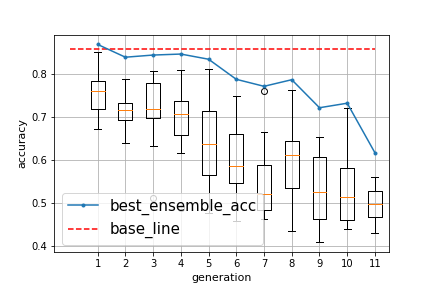
\includegraphics[scale=0.6]{graph_5.png}
	\caption{$\alpha =1.5$の推移\label{fig:graph2}}
\end{figure}

\begin{figure}[h]
	\centering
	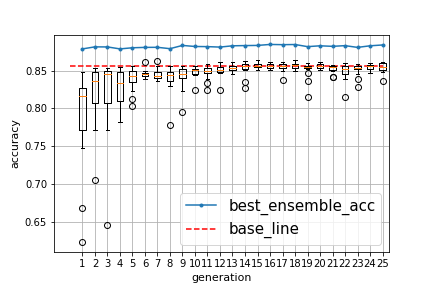
\includegraphics[scale=0.6]{graph_6.png}
	\caption{$\alpha =0.9$の推移\label{fig:graph3}}
\end{figure}

\begin{figure}[h]
	\centering
	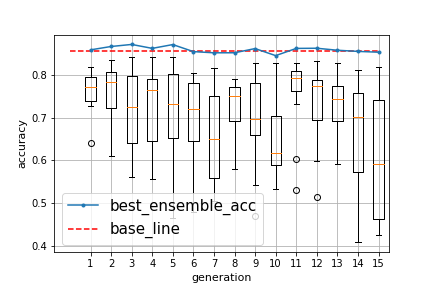
\includegraphics[scale=0.6]{graph_7.png}
	\caption{$\alpha =1.1$の推移\label{fig:graph4}}
\end{figure}

\begin{figure}[p]
	\centering
	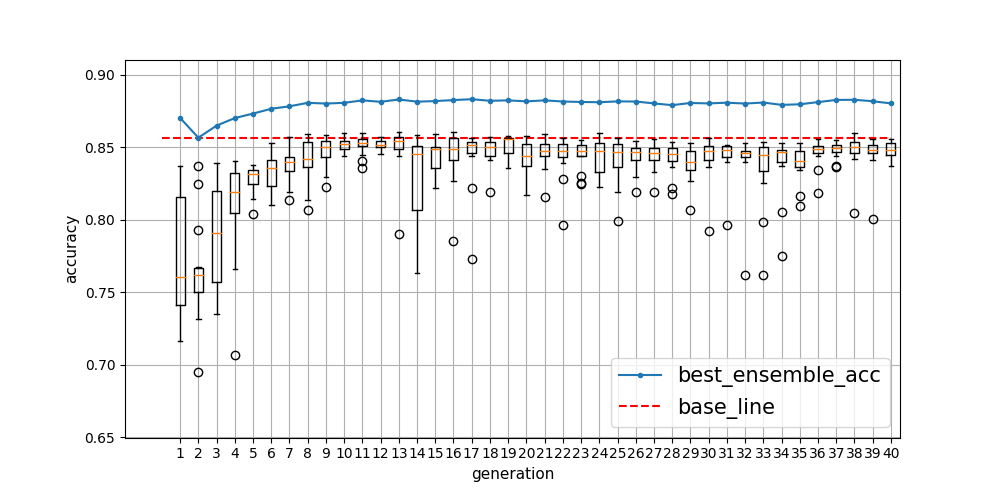
\includegraphics[scale=0.8]{graph_4.png}
	\caption{$\alpha =1$の推移\label{fig:graph1}}
\end{figure}

\end{document}


